\subsection{Maquette}

Les images \ref{maquette1} et \ref{maquette2} représentent la maquette permettant de décrire le cahier des charges et les spécifications d'interface qui ont été fourni pour la réalisation de l'application.

\begin{figure}[!h]
	\begin{center}
		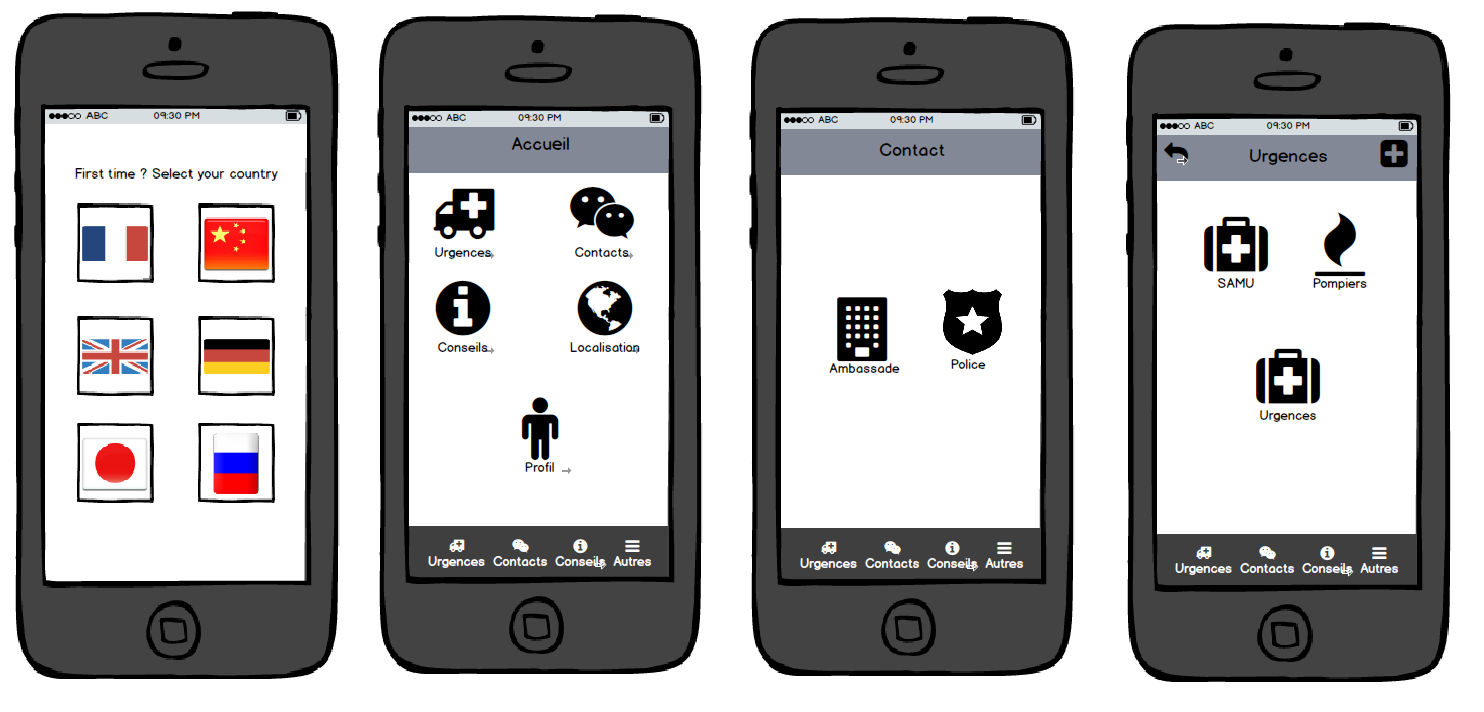
\includegraphics[scale=0.45]{img/maquette1.png}
		\caption{Maquette de l'application}
		\label{maquette1} 
	\end{center}
\end{figure}

\begin{figure}[!h]
	\begin{center}
		
		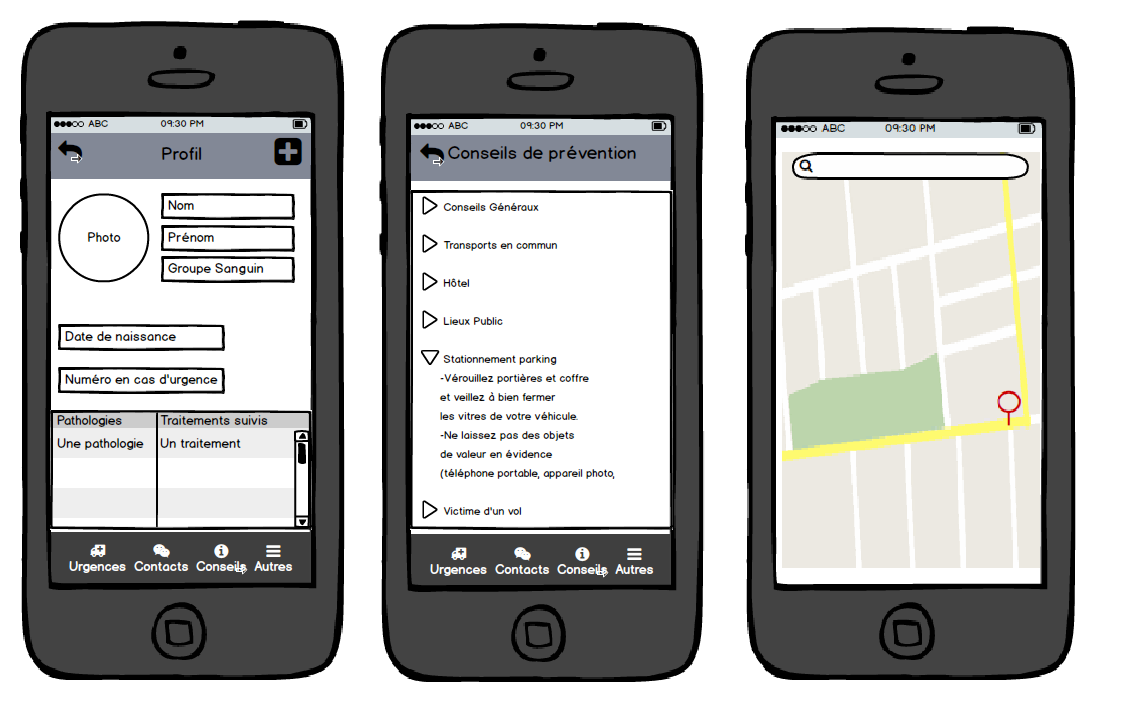
\includegraphics[scale=0.5]{img/maquette2.png}
		\caption{Maquette de l'application : }
		\label{maquette2} 
		
	\end{center}
\end{figure}